\documentclass{beamer}

\usefonttheme{serif}

\usepackage{graphicx}
\usepackage{xcolor}
\usepackage{tikz}
\usepackage{amsmath}
\usepackage{physics}
\usepackage{siunitx}
\usepackage{hyperref}
\usepackage{listings}

\usetikzlibrary{positioning, arrows.meta}

\hypersetup{
    colorlinks=true,
    linkcolor=blue,
    urlcolor=blue
}

\definecolor{blue}{rgb}{0.0234375,0.11328125,0.609375}

\setbeamercolor{frametitle}{fg=blue}
\setbeamercolor{title}{fg=blue}
\setbeamercolor{structure}{fg=blue}


\title{\textcolor{blue}{Robust Edge Detection for Robot Vision}}

\subtitle{
\textcolor{blue}{
Image Processing Project\\
Data and Compute Intensive Sciences Research Group
}
}

\author{
Balázs, Paszkál, Vince, Levente, Bence, Antal\\
Éva, Hajni
}

\date{\textcolor{blue}{6-10 July 2026}}


\setbeamertemplate{footline}{
\leavevmode%
\hbox{
\begin{beamercolorbox}[wd=.1\paperwidth,ht=2.25ex,dp=1ex,left]{page number in head/foot}
\hspace{1em}\textcolor{blue}{\insertframenumber}
\end{beamercolorbox}}
\vskip0pt
}


\AtBeginSection[]
{
\begin{frame}{Outline}
\tableofcontents[currentsection]
\end{frame}
}


\begin{document}


%------------------------------------------------

\begin{frame}

    \titlepage

    \begin{center}
        
\includegraphics[width=0.25\textwidth]{img/logo.png}
    \end{center}

\end{frame}


%------------------------------------------------

\section{Motivation}


\begin{frame}{Why Do Machines Need Vision?}

    Modern robots need to understand their environment.

    \begin{itemize}
        \item Autonomous vehicles
        \item Warehouse robots
        \item Drones
        \item Industrial systems
    \end{itemize}

    \vspace{0.3cm}

    A camera only provides pixels.

    \textbf{How can we extract useful information from images?}

\end{frame}



%------------------------------------------------


\begin{frame}{From Image to Information}

    \begin{columns}

        \column{0.5\textwidth}

        
\includegraphics[width=\textwidth]{img/result_original.png}


        \column{0.5\textwidth}

        \begin{itemize}

            \item Raw image contains millions of values

            \item Important structures are hidden

            \item We search for:
                  \begin{itemize}
                      \item edges
                      \item shapes
                      \item movement
                  \end{itemize}

        \end{itemize}

    \end{columns}

\end{frame}



%------------------------------------------------

\section{The Problem}


\begin{frame}{Classical Edge Detection}


    One common method is the Canny edge detector.

    \vspace{0.4cm}


    \begin{center}

        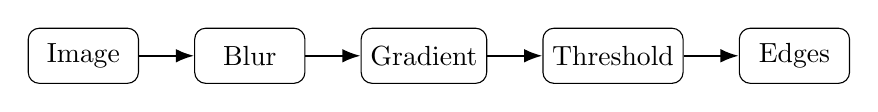
\begin{tikzpicture}[
                node distance=0.7cm,
                every node/.style={
                        draw,
                        rounded corners,
                        minimum width=1.4cm,
                        minimum height=0.7cm,
                        align=center
                    }
            ]


            \node (a) {Image};
            \node (b) [right=of a] {Blur};
            \node (c) [right=of b] {Gradient};
            \node (d) [right=of c] {Threshold};
            \node (e) [right=of d] {Edges};


            \draw[-{Latex}, thick] (a)--(b);
            \draw[-{Latex}, thick] (b)--(c);
            \draw[-{Latex}, thick] (c)--(d);
            \draw[-{Latex}, thick] (d)--(e);


        \end{tikzpicture}

    \end{center}


\end{frame}



%------------------------------------------------


\begin{frame}{The Limitation}


    Classical methods can be unstable.

    \vspace{0.4cm}


    \begin{columns}


        \column{0.5\textwidth}

        
\includegraphics[width=\textwidth]{img/too_many_edges.png}

        Too many edges


        \column{0.5\textwidth}

        
\includegraphics[width=\textwidth]{img/missing_edges.png}

        Missing edges


    \end{columns}


\end{frame}



%------------------------------------------------


\begin{frame}{Our Goal}


    We want a method that:

    \begin{itemize}

        \item Detects important structures

        \item Ignores noise

        \item Works with real camera input

        \item Is robust in changing conditions

    \end{itemize}


\end{frame}



%------------------------------------------------

\section{Our Method}


\begin{frame}{Convolution Based Approach}


    Images can be processed using convolution kernels.


    \[
        \begin{bmatrix}
            -1 & -1 & -1 \\
            0  & 0  & 0  \\
            1  & 1  & 1
        \end{bmatrix}
    \]


    The kernel scans the image and detects patterns.


\end{frame}



%------------------------------------------------


\begin{frame}{How Convolution Works}


    \begin{center}

        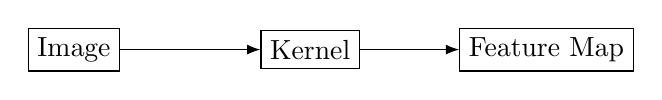
\begin{tikzpicture}

            \node[draw] (a) at (0,0) {Image};

            \node[draw] (b) at (3,0) {Kernel};

            \node[draw] (c) at (6,0) {Feature Map};


            \draw[-{Latex}] (a)--(b);
            \draw[-{Latex}] (b)--(c);

        \end{tikzpicture}

    \end{center}


    The result highlights important information.

\end{frame}



%------------------------------------------------

\section{Results}


\begin{frame}{Example Results}


    \begin{columns}


        \column{0.33\textwidth}

        
\includegraphics[width=\textwidth]{img/result_original.png}

        Original


        \column{0.33\textwidth}

        
\includegraphics[width=\textwidth]{img/result_canny.png}

        Canny


        \column{0.33\textwidth}

        
\includegraphics[width=\textwidth]{img/result_method.png}

        Our method


    \end{columns}


\end{frame}



%------------------------------------------------


\begin{frame}{Applications}


    Applications:

    \begin{itemize}

        \item Robot vision

        \item Video stabilization

        \item Distance measurement

        \item Object tracking

        \item Autonomous systems

    \end{itemize}


\end{frame}



%------------------------------------------------

\section{Summer Camp Project}


\begin{frame}{What We Do During The Camp}


    \begin{enumerate}

        \item Introduction to image processing

        \item Understanding convolution methods

        \item Implementing edge detection

        \item Applying methods to robot camera

        \item Video stabilization experiments

        \item Evaluation of results


    \end{enumerate}


\end{frame}



%------------------------------------------------


\begin{frame}{Final Goal}


    Build a system that can:


    \begin{center}

        \textbf{See → Understand → React}

    \end{center}


    using real camera data.


\end{frame}


\end{document}